% Options for packages loaded elsewhere
\PassOptionsToPackage{unicode}{hyperref}
\PassOptionsToPackage{hyphens}{url}
%
\documentclass[
  ignorenonframetext,
]{beamer}
\usepackage{pgfpages}
\setbeamertemplate{caption}[numbered]
\setbeamertemplate{caption label separator}{: }
\setbeamercolor{caption name}{fg=normal text.fg}
\beamertemplatenavigationsymbolsempty
% Prevent slide breaks in the middle of a paragraph
\widowpenalties 1 10000
\raggedbottom
\setbeamertemplate{part page}{
  \centering
  \begin{beamercolorbox}[sep=16pt,center]{part title}
    \usebeamerfont{part title}\insertpart\par
  \end{beamercolorbox}
}
\setbeamertemplate{section page}{
  \centering
  \begin{beamercolorbox}[sep=12pt,center]{part title}
    \usebeamerfont{section title}\insertsection\par
  \end{beamercolorbox}
}
\setbeamertemplate{subsection page}{
  \centering
  \begin{beamercolorbox}[sep=8pt,center]{part title}
    \usebeamerfont{subsection title}\insertsubsection\par
  \end{beamercolorbox}
}
\AtBeginPart{
  \frame{\partpage}
}
\AtBeginSection{
  \ifbibliography
  \else
    \frame{\sectionpage}
  \fi
}
\AtBeginSubsection{
  \frame{\subsectionpage}
}

\usepackage{amsmath,amssymb}
\usepackage{iftex}
\ifPDFTeX
  \usepackage[T1]{fontenc}
  \usepackage[utf8]{inputenc}
  \usepackage{textcomp} % provide euro and other symbols
\else % if luatex or xetex
  \usepackage{unicode-math}
  \defaultfontfeatures{Scale=MatchLowercase}
  \defaultfontfeatures[\rmfamily]{Ligatures=TeX,Scale=1}
\fi
\usepackage{lmodern}
\ifPDFTeX\else  
    % xetex/luatex font selection
\fi
% Use upquote if available, for straight quotes in verbatim environments
\IfFileExists{upquote.sty}{\usepackage{upquote}}{}
\IfFileExists{microtype.sty}{% use microtype if available
  \usepackage[]{microtype}
  \UseMicrotypeSet[protrusion]{basicmath} % disable protrusion for tt fonts
}{}
\makeatletter
\@ifundefined{KOMAClassName}{% if non-KOMA class
  \IfFileExists{parskip.sty}{%
    \usepackage{parskip}
  }{% else
    \setlength{\parindent}{0pt}
    \setlength{\parskip}{6pt plus 2pt minus 1pt}}
}{% if KOMA class
  \KOMAoptions{parskip=half}}
\makeatother
\usepackage{xcolor}
\newif\ifbibliography
\setlength{\emergencystretch}{3em} % prevent overfull lines
\setcounter{secnumdepth}{-\maxdimen} % remove section numbering

\usepackage{color}
\usepackage{fancyvrb}
\newcommand{\VerbBar}{|}
\newcommand{\VERB}{\Verb[commandchars=\\\{\}]}
\DefineVerbatimEnvironment{Highlighting}{Verbatim}{commandchars=\\\{\}}
% Add ',fontsize=\small' for more characters per line
\usepackage{framed}
\definecolor{shadecolor}{RGB}{241,243,245}
\newenvironment{Shaded}{\begin{snugshade}}{\end{snugshade}}
\newcommand{\AlertTok}[1]{\textcolor[rgb]{0.68,0.00,0.00}{#1}}
\newcommand{\AnnotationTok}[1]{\textcolor[rgb]{0.37,0.37,0.37}{#1}}
\newcommand{\AttributeTok}[1]{\textcolor[rgb]{0.40,0.45,0.13}{#1}}
\newcommand{\BaseNTok}[1]{\textcolor[rgb]{0.68,0.00,0.00}{#1}}
\newcommand{\BuiltInTok}[1]{\textcolor[rgb]{0.00,0.23,0.31}{#1}}
\newcommand{\CharTok}[1]{\textcolor[rgb]{0.13,0.47,0.30}{#1}}
\newcommand{\CommentTok}[1]{\textcolor[rgb]{0.37,0.37,0.37}{#1}}
\newcommand{\CommentVarTok}[1]{\textcolor[rgb]{0.37,0.37,0.37}{\textit{#1}}}
\newcommand{\ConstantTok}[1]{\textcolor[rgb]{0.56,0.35,0.01}{#1}}
\newcommand{\ControlFlowTok}[1]{\textcolor[rgb]{0.00,0.23,0.31}{\textbf{#1}}}
\newcommand{\DataTypeTok}[1]{\textcolor[rgb]{0.68,0.00,0.00}{#1}}
\newcommand{\DecValTok}[1]{\textcolor[rgb]{0.68,0.00,0.00}{#1}}
\newcommand{\DocumentationTok}[1]{\textcolor[rgb]{0.37,0.37,0.37}{\textit{#1}}}
\newcommand{\ErrorTok}[1]{\textcolor[rgb]{0.68,0.00,0.00}{#1}}
\newcommand{\ExtensionTok}[1]{\textcolor[rgb]{0.00,0.23,0.31}{#1}}
\newcommand{\FloatTok}[1]{\textcolor[rgb]{0.68,0.00,0.00}{#1}}
\newcommand{\FunctionTok}[1]{\textcolor[rgb]{0.28,0.35,0.67}{#1}}
\newcommand{\ImportTok}[1]{\textcolor[rgb]{0.00,0.46,0.62}{#1}}
\newcommand{\InformationTok}[1]{\textcolor[rgb]{0.37,0.37,0.37}{#1}}
\newcommand{\KeywordTok}[1]{\textcolor[rgb]{0.00,0.23,0.31}{\textbf{#1}}}
\newcommand{\NormalTok}[1]{\textcolor[rgb]{0.00,0.23,0.31}{#1}}
\newcommand{\OperatorTok}[1]{\textcolor[rgb]{0.37,0.37,0.37}{#1}}
\newcommand{\OtherTok}[1]{\textcolor[rgb]{0.00,0.23,0.31}{#1}}
\newcommand{\PreprocessorTok}[1]{\textcolor[rgb]{0.68,0.00,0.00}{#1}}
\newcommand{\RegionMarkerTok}[1]{\textcolor[rgb]{0.00,0.23,0.31}{#1}}
\newcommand{\SpecialCharTok}[1]{\textcolor[rgb]{0.37,0.37,0.37}{#1}}
\newcommand{\SpecialStringTok}[1]{\textcolor[rgb]{0.13,0.47,0.30}{#1}}
\newcommand{\StringTok}[1]{\textcolor[rgb]{0.13,0.47,0.30}{#1}}
\newcommand{\VariableTok}[1]{\textcolor[rgb]{0.07,0.07,0.07}{#1}}
\newcommand{\VerbatimStringTok}[1]{\textcolor[rgb]{0.13,0.47,0.30}{#1}}
\newcommand{\WarningTok}[1]{\textcolor[rgb]{0.37,0.37,0.37}{\textit{#1}}}

\providecommand{\tightlist}{%
  \setlength{\itemsep}{0pt}\setlength{\parskip}{0pt}}\usepackage{longtable,booktabs,array}
\usepackage{calc} % for calculating minipage widths
\usepackage{caption}
% Make caption package work with longtable
\makeatletter
\def\fnum@table{\tablename~\thetable}
\makeatother
\usepackage{graphicx}
\makeatletter
\def\maxwidth{\ifdim\Gin@nat@width>\linewidth\linewidth\else\Gin@nat@width\fi}
\def\maxheight{\ifdim\Gin@nat@height>\textheight\textheight\else\Gin@nat@height\fi}
\makeatother
% Scale images if necessary, so that they will not overflow the page
% margins by default, and it is still possible to overwrite the defaults
% using explicit options in \includegraphics[width, height, ...]{}
\setkeys{Gin}{width=\maxwidth,height=\maxheight,keepaspectratio}
% Set default figure placement to htbp
\makeatletter
\def\fps@figure{htbp}
\makeatother

\makeatletter
\@ifpackageloaded{caption}{}{\usepackage{caption}}
\AtBeginDocument{%
\ifdefined\contentsname
  \renewcommand*\contentsname{Table of contents}
\else
  \newcommand\contentsname{Table of contents}
\fi
\ifdefined\listfigurename
  \renewcommand*\listfigurename{List of Figures}
\else
  \newcommand\listfigurename{List of Figures}
\fi
\ifdefined\listtablename
  \renewcommand*\listtablename{List of Tables}
\else
  \newcommand\listtablename{List of Tables}
\fi
\ifdefined\figurename
  \renewcommand*\figurename{Figure}
\else
  \newcommand\figurename{Figure}
\fi
\ifdefined\tablename
  \renewcommand*\tablename{Table}
\else
  \newcommand\tablename{Table}
\fi
}
\@ifpackageloaded{float}{}{\usepackage{float}}
\floatstyle{ruled}
\@ifundefined{c@chapter}{\newfloat{codelisting}{h}{lop}}{\newfloat{codelisting}{h}{lop}[chapter]}
\floatname{codelisting}{Listing}
\newcommand*\listoflistings{\listof{codelisting}{List of Listings}}
\makeatother
\makeatletter
\makeatother
\makeatletter
\@ifpackageloaded{caption}{}{\usepackage{caption}}
\@ifpackageloaded{subcaption}{}{\usepackage{subcaption}}
\makeatother
\ifLuaTeX
  \usepackage{selnolig}  % disable illegal ligatures
\fi
\usepackage{bookmark}

\IfFileExists{xurl.sty}{\usepackage{xurl}}{} % add URL line breaks if available
\urlstyle{same} % disable monospaced font for URLs
\hypersetup{
  pdftitle={ASP.NET (MVC e-commerce)},
  pdfauthor={Patrik Kenfack},
  hidelinks,
  pdfcreator={LaTeX via pandoc}}

\title{ASP.NET (MVC e-commerce)}
\subtitle{React - LINQ - Entity Frame Work - MS SqlServer}
\author{Patrik Kenfack}
\date{}

\begin{document}
\frame{\titlepage}

\begin{frame}
\begin{block}{Plan}
\phantomsection\label{plan}
\begin{itemize}
\tightlist
\item
  Rappel sur la programmation web
\item
  Architecture MVC (Model - Vue - Controleur)

  \begin{itemize}
  \tightlist
  \item
    Motivations
  \item
    Strutures et Normes
  \item
    Mise en place
  \end{itemize}
\item
  Technologies utilisés

  \begin{itemize}
  \tightlist
  \item
    ASP.NET
  \item
    Entity FrameWork (EF)
  \item
    MS SQLServer
  \item
    React
  \item
    LINQ
  \end{itemize}
\end{itemize}
\end{block}
\end{frame}

\begin{frame}{Ceci est un aperçu\ldots{}}
\phantomsection\label{ceci-est-un-aperuxe7u}
\end{frame}

\begin{frame}{Objectif du cours.}
\phantomsection\label{objectif-du-cours.}
À l'issue de ce cours l'étudiant doit être capable de:

\begin{itemize}
\tightlist
\item
  Définir et motiver l'achitecture MVC
\item
  Comprendre la position de differentes technologies dans le model MVC.
\item
  Connaîtres les normes et contraintes du model MVC dans le
  developpement web.
\end{itemize}
\end{frame}

\begin{frame}{La programmation web}
\phantomsection\label{la-programmation-web}
\begin{block}{La programmation web}
\phantomsection\label{la-programmation-web-1}
\begin{itemize}[<+->]
\tightlist
\item
  Créer des sitewebs dynamiques\\
\item
  Code serveur (backend)
\item
  Code client (frontend)
\item
  Traiter les données, afficher le contenu et interagir avec les
  utilisateurs.
\end{itemize}
\end{block}
\end{frame}

\begin{frame}
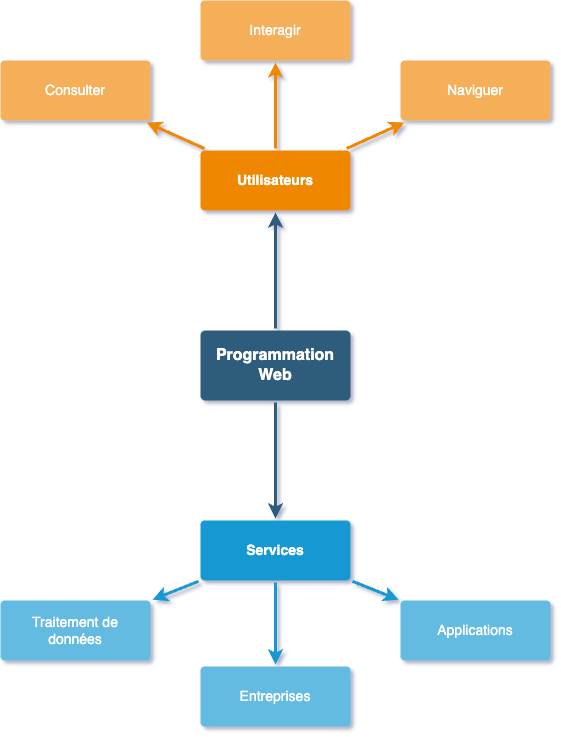
\includegraphics[width=5.10417in,height=\textheight]{./images/Overview_web_programming-Page-2.png}

\begin{block}{La programmation web}
\phantomsection\label{la-programmation-web-2}
\end{block}
\end{frame}

\begin{frame}
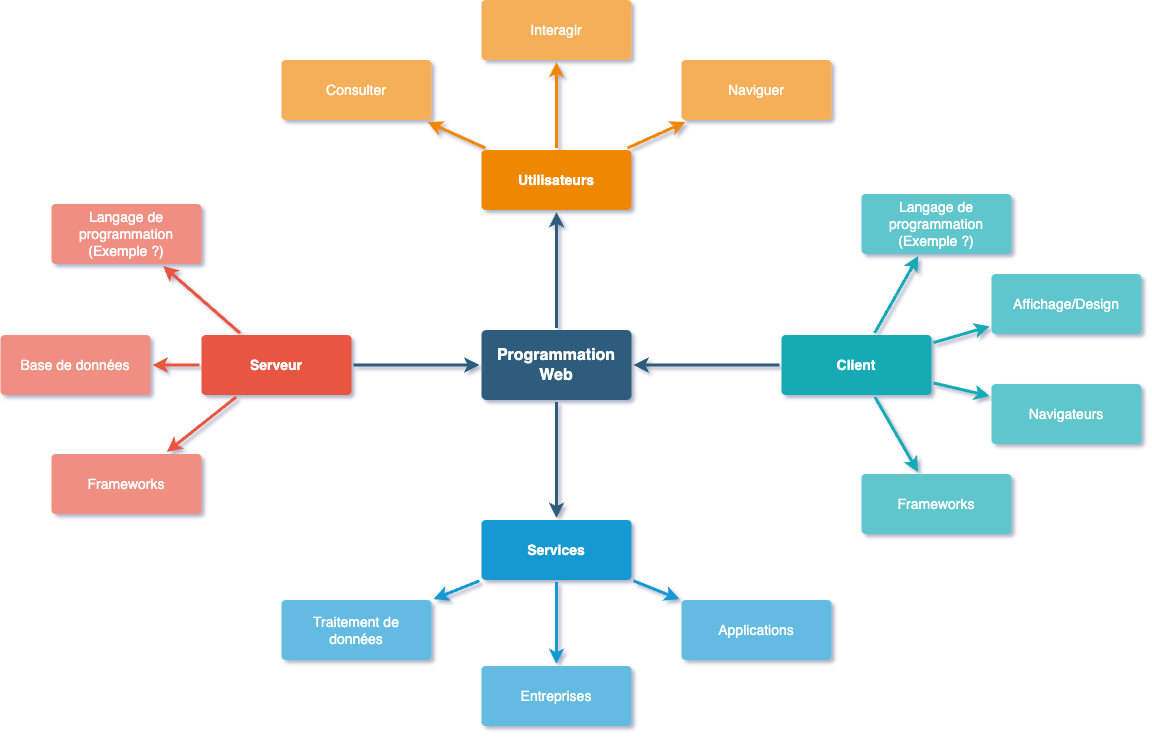
\includegraphics[width=14.58333in,height=\textheight]{./images/Overview_web_programming-Page-1.png}

\begin{block}{La programmation web}
\phantomsection\label{la-programmation-web-3}
\end{block}
\end{frame}

\begin{frame}[fragile]{Architecture MVC}
\phantomsection\label{architecture-mvc}
\begin{block}{Example}
\phantomsection\label{example}
Page ASP presentant la liste des produits (\texttt{Default.aspx})

\begin{Shaded}
\begin{Highlighting}[]
\ErrorTok{\textless{}}\NormalTok{\%@ Page Language="C\#" AutoEventWireup="true" CodeFile="Default.aspx.cs" Inherits="\_Default" \%\textgreater{}}

\DataTypeTok{\textless{}!DOCTYPE}\NormalTok{ html}\DataTypeTok{\textgreater{}}
\DataTypeTok{\textless{}}\KeywordTok{html}\OtherTok{ lang}\OperatorTok{=}\StringTok{"en"}\DataTypeTok{\textgreater{}}
\DataTypeTok{\textless{}}\KeywordTok{head}\DataTypeTok{\textgreater{}}
    \DataTypeTok{\textless{}}\KeywordTok{meta}\OtherTok{ charset}\OperatorTok{=}\StringTok{"UTF{-}8"}\DataTypeTok{\textgreater{}}
    \DataTypeTok{\textless{}}\KeywordTok{title}\DataTypeTok{\textgreater{}}\NormalTok{Product List}\DataTypeTok{\textless{}/}\KeywordTok{title}\DataTypeTok{\textgreater{}}
\DataTypeTok{\textless{}/}\KeywordTok{head}\DataTypeTok{\textgreater{}}
\DataTypeTok{\textless{}}\KeywordTok{body}\DataTypeTok{\textgreater{}}
    \DataTypeTok{\textless{}}\KeywordTok{h1}\DataTypeTok{\textgreater{}}\NormalTok{Product List}\DataTypeTok{\textless{}/}\KeywordTok{h1}\DataTypeTok{\textgreater{}}
    \DataTypeTok{\textless{}}\KeywordTok{asp:GridView}\OtherTok{ ID}\OperatorTok{=}\StringTok{"GridView1"}\OtherTok{ runat}\OperatorTok{=}\StringTok{"server"}\DataTypeTok{\textgreater{}\textless{}/}\KeywordTok{asp:GridView}\DataTypeTok{\textgreater{}}

    \DataTypeTok{\textless{}}\KeywordTok{h2}\DataTypeTok{\textgreater{}}\NormalTok{Add a New Product}\DataTypeTok{\textless{}/}\KeywordTok{h2}\DataTypeTok{\textgreater{}}
    \DataTypeTok{\textless{}}\KeywordTok{form}\OtherTok{ id}\OperatorTok{=}\StringTok{"form1"}\OtherTok{ runat}\OperatorTok{=}\StringTok{"server"}\DataTypeTok{\textgreater{}}
        \DataTypeTok{\textless{}}\KeywordTok{label}\OtherTok{ for}\OperatorTok{=}\StringTok{"txtProductName"}\DataTypeTok{\textgreater{}}\NormalTok{Product Name:}\DataTypeTok{\textless{}/}\KeywordTok{label}\DataTypeTok{\textgreater{}}
        \DataTypeTok{\textless{}}\KeywordTok{asp:TextBox}\OtherTok{ ID}\OperatorTok{=}\StringTok{"txtProductName"}\OtherTok{ runat}\OperatorTok{=}\StringTok{"server"}\DataTypeTok{\textgreater{}\textless{}/}\KeywordTok{asp:TextBox}\DataTypeTok{\textgreater{}}
        \DataTypeTok{\textless{}}\KeywordTok{br}\OtherTok{ }\DataTypeTok{/\textgreater{}}
        \DataTypeTok{\textless{}}\KeywordTok{label}\OtherTok{ for}\OperatorTok{=}\StringTok{"txtPrice"}\DataTypeTok{\textgreater{}}\NormalTok{Price:}\DataTypeTok{\textless{}/}\KeywordTok{label}\DataTypeTok{\textgreater{}}
        \DataTypeTok{\textless{}}\KeywordTok{asp:TextBox}\OtherTok{ ID}\OperatorTok{=}\StringTok{"txtPrice"}\OtherTok{ runat}\OperatorTok{=}\StringTok{"server"}\DataTypeTok{\textgreater{}\textless{}/}\KeywordTok{asp:TextBox}\DataTypeTok{\textgreater{}}
        \DataTypeTok{\textless{}}\KeywordTok{br}\OtherTok{ }\DataTypeTok{/\textgreater{}}
        \DataTypeTok{\textless{}}\KeywordTok{asp:Button}\OtherTok{ ID}\OperatorTok{=}\StringTok{"btnAddProduct"}\OtherTok{ runat}\OperatorTok{=}\StringTok{"server"}\OtherTok{ Text}\OperatorTok{=}\StringTok{"Add Product"}\OtherTok{ OnClick}\OperatorTok{=}\StringTok{"btnAddProduct\_Click"}\OtherTok{ }\DataTypeTok{/\textgreater{}}
    \DataTypeTok{\textless{}/}\KeywordTok{form}\DataTypeTok{\textgreater{}}
\DataTypeTok{\textless{}/}\KeywordTok{body}\DataTypeTok{\textgreater{}}
\DataTypeTok{\textless{}/}\KeywordTok{html}\DataTypeTok{\textgreater{}}
\end{Highlighting}
\end{Shaded}
\end{block}

\begin{block}{Example}
\phantomsection\label{example-1}
Fichier \texttt{Default.aspx.cs}

\begin{Shaded}
\begin{Highlighting}[]
\KeywordTok{using}\NormalTok{ System}\OperatorTok{;}
\KeywordTok{using}\NormalTok{ System}\OperatorTok{.}\FunctionTok{Data}\OperatorTok{;}
\KeywordTok{using}\NormalTok{ System}\OperatorTok{.}\FunctionTok{Data}\OperatorTok{.}\FunctionTok{SqlClient}\OperatorTok{;}
\KeywordTok{using}\NormalTok{ System}\OperatorTok{.}\FunctionTok{Configuration}\OperatorTok{;}

\KeywordTok{public} \KeywordTok{partial} \KeywordTok{class}\NormalTok{ \_Default }\OperatorTok{:}\NormalTok{ System}\OperatorTok{.}\FunctionTok{Web}\OperatorTok{.}\FunctionTok{UI}\OperatorTok{.}\FunctionTok{Page}
\OperatorTok{\{}
    \KeywordTok{protected} \DataTypeTok{void} \FunctionTok{Page\_Load}\OperatorTok{(}\DataTypeTok{object}\NormalTok{ sender}\OperatorTok{,}\NormalTok{ EventArgs e}\OperatorTok{)}
    \OperatorTok{\{}
        \KeywordTok{if} \OperatorTok{(!}\NormalTok{IsPostBack}\OperatorTok{)}
        \OperatorTok{\{}
            \FunctionTok{LoadProducts}\OperatorTok{();}
        \OperatorTok{\}}
    \OperatorTok{\}}

    \KeywordTok{protected} \DataTypeTok{void} \FunctionTok{LoadProducts}\OperatorTok{()}
    \OperatorTok{\{}
        \DataTypeTok{string}\NormalTok{ connString }\OperatorTok{=}\NormalTok{ ConfigurationManager}\OperatorTok{.}\FunctionTok{ConnectionStrings}\OperatorTok{[}\StringTok{"DefaultConnection"}\OperatorTok{].}\FunctionTok{ConnectionString}\OperatorTok{;}
        \DataTypeTok{string}\NormalTok{ query }\OperatorTok{=} \StringTok{"SELECT ProductID, ProductName, Price FROM Products"}\OperatorTok{;}

        \KeywordTok{using} \OperatorTok{(}\NormalTok{SqlConnection conn }\OperatorTok{=} \KeywordTok{new} \FunctionTok{SqlConnection}\OperatorTok{(}\NormalTok{connString}\OperatorTok{))}
        \OperatorTok{\{}
\NormalTok{            SqlCommand cmd }\OperatorTok{=} \KeywordTok{new} \FunctionTok{SqlCommand}\OperatorTok{(}\NormalTok{query}\OperatorTok{,}\NormalTok{ conn}\OperatorTok{);}
\NormalTok{            conn}\OperatorTok{.}\FunctionTok{Open}\OperatorTok{();}

\NormalTok{            SqlDataAdapter da }\OperatorTok{=} \KeywordTok{new} \FunctionTok{SqlDataAdapter}\OperatorTok{(}\NormalTok{cmd}\OperatorTok{);}
\NormalTok{            DataTable dt }\OperatorTok{=} \KeywordTok{new} \FunctionTok{DataTable}\OperatorTok{();}
\NormalTok{            da}\OperatorTok{.}\FunctionTok{Fill}\OperatorTok{(}\NormalTok{dt}\OperatorTok{);}

\NormalTok{            GridView1}\OperatorTok{.}\FunctionTok{DataSource} \OperatorTok{=}\NormalTok{ dt}\OperatorTok{;}
\NormalTok{            GridView1}\OperatorTok{.}\FunctionTok{DataBind}\OperatorTok{();}
        \OperatorTok{\}}
    \OperatorTok{\}}

    \KeywordTok{protected} \DataTypeTok{void} \FunctionTok{btnAddProduct\_Click}\OperatorTok{(}\DataTypeTok{object}\NormalTok{ sender}\OperatorTok{,}\NormalTok{ EventArgs e}\OperatorTok{)}
    \OperatorTok{\{}
        \DataTypeTok{string}\NormalTok{ productName }\OperatorTok{=}\NormalTok{ txtProductName}\OperatorTok{.}\FunctionTok{Text}\OperatorTok{;}
        \DataTypeTok{decimal}\NormalTok{ price}\OperatorTok{;}

        \KeywordTok{if} \OperatorTok{(}\DataTypeTok{string}\OperatorTok{.}\FunctionTok{IsNullOrWhiteSpace}\OperatorTok{(}\NormalTok{productName}\OperatorTok{)} \OperatorTok{||} \OperatorTok{!}\DataTypeTok{decimal}\OperatorTok{.}\FunctionTok{TryParse}\OperatorTok{(}\NormalTok{txtPrice}\OperatorTok{.}\FunctionTok{Text}\OperatorTok{,} \KeywordTok{out}\NormalTok{ price}\OperatorTok{))}
        \OperatorTok{\{}
            \CommentTok{// Display error message (in a real{-}world scenario)}
            \KeywordTok{return}\OperatorTok{;}
        \OperatorTok{\}}

        \DataTypeTok{string}\NormalTok{ connString }\OperatorTok{=}\NormalTok{ ConfigurationManager}\OperatorTok{.}\FunctionTok{ConnectionStrings}\OperatorTok{[}\StringTok{"DefaultConnection"}\OperatorTok{].}\FunctionTok{ConnectionString}\OperatorTok{;}
        \DataTypeTok{string}\NormalTok{ query }\OperatorTok{=} \StringTok{"INSERT INTO Products (ProductName, Price) VALUES (@ProductName, @Price)"}\OperatorTok{;}

        \KeywordTok{using} \OperatorTok{(}\NormalTok{SqlConnection conn }\OperatorTok{=} \KeywordTok{new} \FunctionTok{SqlConnection}\OperatorTok{(}\NormalTok{connString}\OperatorTok{))}
        \OperatorTok{\{}
\NormalTok{            SqlCommand cmd }\OperatorTok{=} \KeywordTok{new} \FunctionTok{SqlCommand}\OperatorTok{(}\NormalTok{query}\OperatorTok{,}\NormalTok{ conn}\OperatorTok{);}
\NormalTok{            cmd}\OperatorTok{.}\FunctionTok{Parameters}\OperatorTok{.}\FunctionTok{AddWithValue}\OperatorTok{(}\StringTok{"@ProductName"}\OperatorTok{,}\NormalTok{ productName}\OperatorTok{);}
\NormalTok{            cmd}\OperatorTok{.}\FunctionTok{Parameters}\OperatorTok{.}\FunctionTok{AddWithValue}\OperatorTok{(}\StringTok{"@Price"}\OperatorTok{,}\NormalTok{ price}\OperatorTok{);}
\NormalTok{            conn}\OperatorTok{.}\FunctionTok{Open}\OperatorTok{();}
\NormalTok{            cmd}\OperatorTok{.}\FunctionTok{ExecuteNonQuery}\OperatorTok{();}
        \OperatorTok{\}}

        \CommentTok{// Reload the product list}
        \FunctionTok{LoadProducts}\OperatorTok{();}
    \OperatorTok{\}}
\OperatorTok{\}}
\end{Highlighting}
\end{Shaded}
\end{block}

\begin{block}{Model - Vue - Controleur}
\phantomsection\label{model---vue---controleur}
\begin{itemize}
\tightlist
\item
  Quel sont les limites de la programmation web procedurale?
\item
  Drink coffee
\end{itemize}
\end{block}
\end{frame}

\begin{frame}{In the evening}
\phantomsection\label{in-the-evening}
\begin{block}{Dinner}
\phantomsection\label{dinner}
\begin{itemize}
\tightlist
\item
  Eat spaghetti
\item
  Drink wine
\end{itemize}
\end{block}

\begin{block}{Going to sleep}
\phantomsection\label{going-to-sleep}
\begin{itemize}
\tightlist
\item
  Get in bed
\item
  Count sheep
\end{itemize}
\end{block}
\end{frame}



\end{document}
